\section{Statisk temperatur i vägg}

För att beskriva ett värmeflöde används ekvationerna Fouriers värmeekvation
\eqref{eq:staticwallmethod:fourier} och värmeledningsekvationen 
\eqref{eq:staticwallmethod:heat}. 
I dessa är
$k$ värmeledningsförmågan\\i $\mbox{W}\mbox{m}^{-2}\mbox{K}^{-1}$ och
$\alpha$ är termisk diffusivitet i $\mbox{m}^2\mbox{s}^{-1}$. \cite{physicshandbook}

Vid statiskt värmeflöde kommer temperaturderivatan med avseende på tiden att vara noll.
Detta innebär att värmeledningsekvationen övergår i Laplaces ekvation
$\Delta{}T = 0$. I en dimension blir detta $d^2T/dx^2 = 0$ vilket innebär
att lösningen blir ett polynom av första ordningen.  

\begin{equation}
\label{eq:staticwallmethod:fourier}
q_x = -k\frac{dT}{dx}
\end{equation}

\begin{equation}
\label{eq:staticwallmethod:heat}
\frac{\partial{}T}{\partial{}t} = \alpha\Delta{}T
\end{equation}

\begin{figure}
\centering
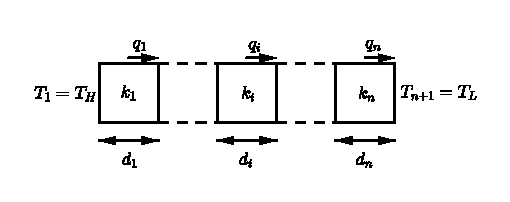
\includegraphics{images/wall.eps}
\caption{Schematisk bild över en vägg som består av $n$ olika element med olika
längd och värmeledningskapacitet.}\label{fig:staticwallmethod:wall}
\end{figure}

\noindent
Vi vill nu beskriva det statiska värmeflödet genom en vägg som består
av flera olika material. De enda värmekällorna som påverkar väggen
är en isoterm $T = T_H$ på ena sidan av väggen
samt en isoterm $T = T_L$ på andra sidan av väggen.

För att göra beräkningarna enklare
ser vi väggen som en oändligt stor skiva. Detta innebär att vi kan räkna
på ekvationen i en dimension. 
En schematisk bild över en vägg i en dimension som består av
$n$ olika material kan ses i figur \ref{fig:staticwallmethod:wall}.
Med materialens värmeledningsförmåga, $k_i$, samt längden
på elementen, $L_i$, använder vi nu Fouriers värmeledningsekvation för
att teckna värmeflödet och temperaturerna $T_j$,  $j=0,\,1,\,...\,,\,n$, i punkterna
mellan de olika delarna av väggen med randvillkoren $T_0 = T_H$ samt
$T_n = T_L$.

För varje del av väggen kan vi sätta upp ekvationer från Fouriers ekvation
för värmeflöde. Vi får flöde in i en del enligt \eqref{eq:staticwallmethod:rod} och
flödet ut genom väggen blir detsamma ty temperaturen är konstant. Dessa två
ekvationer låter oss teckna ett ekvationssystem för varje del av väggen
enligt \eqref{eq:staticwalltheory:rodmatrix}. \cite{lewis04}

\begin{equation}
\label{eq:staticwallmethod:rod}
Q = -k\frac{T_{2}-T_{1}}{L}
\end{equation}


\begin{equation}
\label{eq:staticwalltheory:rodmatrix}
\begin{pmatrix}
Q \\
-Q
\end{pmatrix} = 
\frac{k}{L}\begin{pmatrix}
1 & -1 \\
-1 & 1
\end{pmatrix}
\begin{pmatrix}
T_1 \\
T_2
\end{pmatrix}
\end{equation}

\noindent
Vi kan nu teckna dessa ekvationssystem för alla delar av väggen, som skrivs som 
en matris och sedan fylla ut matriserna med nollelement för att slutligen bilda 
en linjärkomination.
Då linjärkombinationen bildas kommer energiflödena i mitten av väggen att
vara noll. Detta överensstämmer väl med att vi har en statisk energifördelning
utan interna värmekällor.
Slutligen får vi ett ekvationsystem enligt ekvation
\eqref{eq:staticwallmethod:full} som enkelt kan lösas. Matrisen $A$ är linjärkombinationen av nollpaddade versioner av \emph{\color{red} Skriv exempel som förklaring på nollpaddade och använd annat ord ex. 'med nollor utfyllda…' eller 'nollutfyllda'.}
Notera att denna matris är singulär men då det är lika många
obekanta som rangen av matrisen är detta inte ett problem.

\begin{equation}
\label{eq:staticwallmethod:full}
\begin{pmatrix}
Q\\0\\...\\0\\-Q
\end{pmatrix} = A
\begin{pmatrix}
T_H\\T_1\\...\\T_{n-1}\\T_L
\end{pmatrix}
\end{equation}
